% Options for packages loaded elsewhere
\PassOptionsToPackage{unicode}{hyperref}
\PassOptionsToPackage{hyphens}{url}
%
\documentclass[
]{article}
\usepackage{lmodern}
\usepackage{amssymb,amsmath}
\usepackage{ifxetex,ifluatex}
\ifnum 0\ifxetex 1\fi\ifluatex 1\fi=0 % if pdftex
  \usepackage[T1]{fontenc}
  \usepackage[utf8]{inputenc}
  \usepackage{textcomp} % provide euro and other symbols
\else % if luatex or xetex
  \usepackage{unicode-math}
  \defaultfontfeatures{Scale=MatchLowercase}
  \defaultfontfeatures[\rmfamily]{Ligatures=TeX,Scale=1}
\fi
% Use upquote if available, for straight quotes in verbatim environments
\IfFileExists{upquote.sty}{\usepackage{upquote}}{}
\IfFileExists{microtype.sty}{% use microtype if available
  \usepackage[]{microtype}
  \UseMicrotypeSet[protrusion]{basicmath} % disable protrusion for tt fonts
}{}
\makeatletter
\@ifundefined{KOMAClassName}{% if non-KOMA class
  \IfFileExists{parskip.sty}{%
    \usepackage{parskip}
  }{% else
    \setlength{\parindent}{0pt}
    \setlength{\parskip}{6pt plus 2pt minus 1pt}}
}{% if KOMA class
  \KOMAoptions{parskip=half}}
\makeatother
\usepackage{xcolor}
\IfFileExists{xurl.sty}{\usepackage{xurl}}{} % add URL line breaks if available
\IfFileExists{bookmark.sty}{\usepackage{bookmark}}{\usepackage{hyperref}}
\hypersetup{
  pdftitle={Plots},
  hidelinks,
  pdfcreator={LaTeX via pandoc}}
\urlstyle{same} % disable monospaced font for URLs
\usepackage[margin=1in]{geometry}
\usepackage{graphicx,grffile}
\makeatletter
\def\maxwidth{\ifdim\Gin@nat@width>\linewidth\linewidth\else\Gin@nat@width\fi}
\def\maxheight{\ifdim\Gin@nat@height>\textheight\textheight\else\Gin@nat@height\fi}
\makeatother
% Scale images if necessary, so that they will not overflow the page
% margins by default, and it is still possible to overwrite the defaults
% using explicit options in \includegraphics[width, height, ...]{}
\setkeys{Gin}{width=\maxwidth,height=\maxheight,keepaspectratio}
% Set default figure placement to htbp
\makeatletter
\def\fps@figure{htbp}
\makeatother
\setlength{\emergencystretch}{3em} % prevent overfull lines
\providecommand{\tightlist}{%
  \setlength{\itemsep}{0pt}\setlength{\parskip}{0pt}}
\setcounter{secnumdepth}{-\maxdimen} % remove section numbering
\usepackage{fvextra}
\usepackage{adjustbox}
\usepackage{tabularx}
\usepackage{graphicx}
\DefineVerbatimEnvironment{Highlighting}{Verbatim}{
  showspaces = false,
  showtabs = false,
  breaklines,
  commandchars=\\\{\}
}

\title{Plots}
\author{}
\date{\vspace{-2.5em}}

\begin{document}
\maketitle

\begin{figure}

{\centering \includegraphics[width=\textwidth,height=\textheight]{/Users/Personal/Dropbox/Mac/Documents/HCT Counterfactuals/covid-vaccine-timeline/archive/generate_vaccine_counterfactual/20230206-170427-bd46e4e9/cumulative_counterfactuals} 

}

\caption{DJ4 Cumulative vaccine counterfactuals}\label{fig:cumul-vacc-cfacts}
\end{figure}

\hypertarget{dj5-table}{%
\subsubsection{DJ5 Table}\label{dj5-table}}

\input{/Users/Personal/Dropbox/Mac/Documents/HCT Counterfactuals/covid-vaccine-timeline/archive/deaths_averted_plot_timeline/20230206-181403-b1c10039/counterfactuals_table.tex}

\begin{figure}

{\centering \includegraphics[width=\textwidth,height=\textheight]{/Users/Personal/Dropbox/Mac/Documents/HCT Counterfactuals/covid-vaccine-timeline/archive/deaths_averted_plot_timeline/20230206-181403-b1c10039/all_tsplot} 

}

\caption{DJ6 Daily deaths per scenario}\label{fig:daily-deaths}
\end{figure}

\begin{figure}

{\centering \includegraphics[width=\textwidth,height=\textheight]{/Users/Personal/Dropbox/Mac/Documents/HCT Counterfactuals/covid-vaccine-timeline/archive/generate_production_counterfactual/20230206-111046-65dc3164/vaccine_production} 

}

\caption{DJ9 Vaccine production assumptions}\label{fig:prod-assumptions}
\end{figure}

\begin{figure}

{\centering 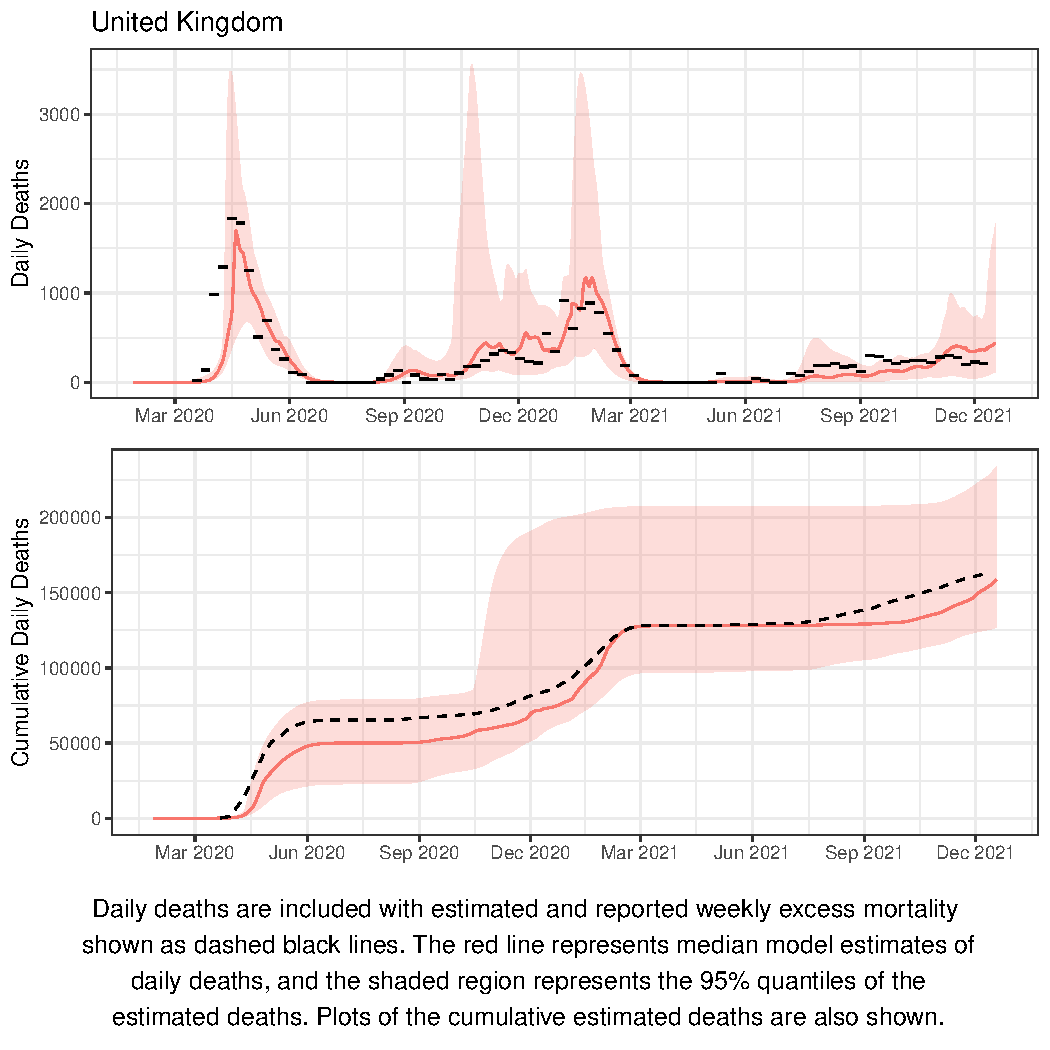
\includegraphics[width=\textwidth,height=\textheight]{/Users/Personal/Dropbox/Mac/Documents/HCT Counterfactuals/covid-vaccine-timeline/archive/generate_vaccine_counterfactual/20230206-170427-bd46e4e9/shifts_plots/GBR} 

}

\caption{DJ10 UK limits from production}\label{fig:GBR-prod-cap}
\end{figure}
\begin{figure}

{\centering 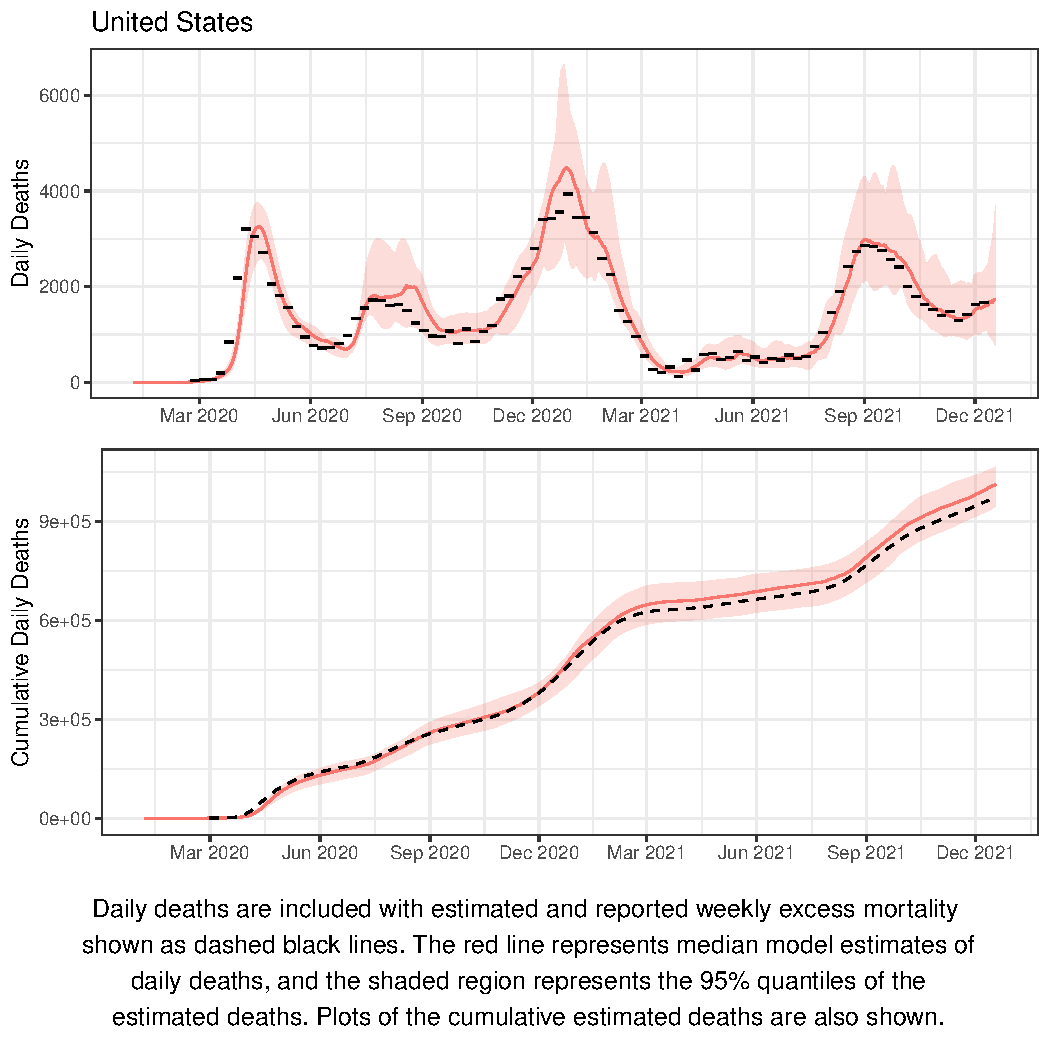
\includegraphics[width=\textwidth,height=\textheight]{/Users/Personal/Dropbox/Mac/Documents/HCT Counterfactuals/covid-vaccine-timeline/archive/generate_vaccine_counterfactual/20230206-170427-bd46e4e9/shifts_plots/USA} 

}

\caption{DJ10 USA limits from production}\label{fig:USA-prod-cap}
\end{figure}

\end{document}
